\begin{title}[\Large]
  Параграф 1.3
\end{title}

\begin{title}[\Large]
  Репер и формулы Френа
\end{title}

\begin{define}[репера Френе]
  $\vec \varphi = \vec \varphi (s)$ регулярная кривая где $s$ натуральный
  параметр

  $\vec t = \frac{d \vec \varphi}{ds}$ касательный вектор

  $\vec n = \frac{1}{k} ~~~ \frac{d^2 \vec \varphi}{ds^2}$ вектор главной
  нормали

  $\vec b = [\vec t, \vec n]$ вектор бинормали

  $\vec t, \vec n, \vec b$ репер Френе (в каждой точке ортонормированный базис)

  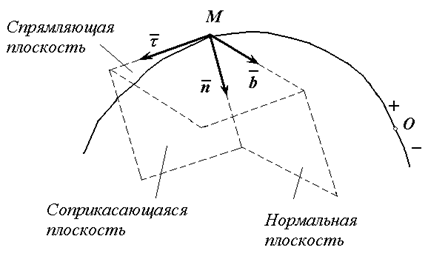
\includegraphics[width = 7cm]{reperFrene}
\end{define}

\begin{block}[Формулы Френе]
  Кривая $\vec \varphi = \vec \varphi(s)$ где $s$ натуральный параметр и
  обозначим
  $$
  \stackrel{\bullet}{\vec \varphi} ~ = \frac{d \vec \varphi}{ds} ~~~
  \stackrel{\bullet \bullet}{\vec \varphi} ~ = \frac{d^2 \vec \varphi}{ds^2} ~~~
  \stackrel{\bullet \bullet \bullet}{\vec \varphi} ~ =
  \frac{d^3 \vec \varphi}{ds^3}
  $$
  тогда
  $$
  \left\{
  \begin{array}{l}
    \stackrel{\bullet}{\vec t} ~ = k \vec n \\
    \stackrel{\bullet}{\vec n} ~ = -k \vec t + \kappa \vec b \\
    \stackrel{\bullet}{\vec b} ~ = - \kappa \vec n
  \end{array}
  \right.
  $$
  $$
  \left(
  \begin{array}{c}
    \stackrel{\bullet}{\vec t} \\
    \stackrel{\bullet}{\vec n} \\
    \stackrel{\bullet}{\vec b}
  \end{array}
  \right) =
  \left(
  \begin{array}{ccc}
    c & k & c \\
    -k & 0 & \kappa \\
    0 & -\kappa & 0
  \end{array}
  \right)
  \left(
  \begin{array}{ccc}
    \vec t \\
    \vec n \\
    \vec b
  \end{array}
  \right)
  $$
\end{block}

\begin{proof}
  $$
  \frac{d\vec t}{ds} = \frac{d^2 \vec \varphi}{ds^2} = k \vec n
  $$
  $$
  \vec b = [\vec t, \vec n] ~~~ \frac{d\vec b}{ds} = - \kappa \vec n
  $$
  $$
  \vec n = [\vec b, \vec t] ~ \Rightarrow ~ \stackrel{\bullet}{\vec n}~ =
  [\stackrel{\bullet}{\vec b}, \vec t] + [\vec b, \stackrel{\bullet}{\vec t}]
  = [-\kappa \vec n, \vec t] + [\vec b, k \vec n] = -\kappa \vec b + k \vec t
  $$
\end{proof}

\begin{title}[\Large]
  Формулы для нахождения кривизны и кручения
\end{title}

\begin{block}[Формулы для нахождения кривезны и кручения кривой]
  $\vec \varphi = \vec \varphi(t)$ регулярная кривая тогда
  $$
  k = \frac{|[\vec \varphi, \vec \varphi'']|}{|\vec \varphi'|^3} ~~~
  \kappa = \frac{( \vec \varphi', \vec \varphi'', \vec \varphi''')}
  {|[\vec \varphi', \vec \varphi'']|^2}
  $$
\end{block}

\begin{proof}
  $$
  \vec \varphi(s) = \vec \varphi(t(s))
  $$
  $$
  \vec t = \stackrel{\bullet}{\vec \varphi} = \frac{d \vec \varphi}{dt}
  \frac{dt}{ds} = \vec \varphi' \frac{dt}{ds}
  $$
  $$
  k \vec n = \stackrel{\bullet \bullet}{\vec \varphi} =
  \stackrel{\bullet}{\vec t} = \vec \varphi'' \left(\frac{dt}{ds}\right)^2 +
  \vec \varphi' \frac{d^2t}{ds^2}
  $$
  $$
  k \vec n - k^2 \vec t + k \kappa \vec b =
  \stackrel{\bullet \bullet \bullet}{\vec \varphi} = \vec \varphi'''
  \left(\frac{dt}{ds}\right)^3 + \vec \varphi'' 2 \frac{dt}{ds}
  \frac{d^2 t}{ds^2} +
  \vec \varphi'' \frac{dt}{ds} \frac{d^2 t}{ds^2} + \vec \varphi'
  \frac{d^3 t}{ds^3} =
  $$
  $$
  = \vec \varphi''' \left(\frac{dt}{ds}\right)^3 + 3 \vec \varphi''
  \frac{dt}{ds}\frac{d^2t}{ds^2} + \vec \varphi' \frac{d^3t}{ds^3}
  $$
  расмотрим $[\stackrel{\bullet}{\vec \varphi},
  \stackrel{\bullet \bullet}{\vec \varphi}]$
  $$
  k \vec b = [\stackrel{\bullet}{\vec \varphi},
  \stackrel{\bullet \bullet}{\vec \varphi}] = \left(\frac{dt}{ds}\right)^3
  [\vec \varphi', \vec \varphi''] = \frac{1}{|\vec \varphi'|^3}
  [\vec \varphi', \vec \varphi'']
  $$
  $$
  s = \int_{t_0}^t |\vec \varphi'|dt ~ \Rightarrow ~ \frac{ds}{dt} =
  |\vec \varphi'| ~ \Rightarrow ~
  k = \frac{|[\vec \varphi, \vec \varphi'']|}{|\vec \varphi'|^3}
  $$
  $$
  (\stackrel{\bullet}{\vec \varphi},
  \stackrel{\bullet \bullet}{\vec \varphi},
  \stackrel{\bullet \bullet \bullet}{\vec \varphi}) = (\vec t, k \vec n,
  k \vec n - R^2t + k \kappa \vec b) = k^2 \kappa(\vec t, \vec n, \vec b) =
  k^2 \kappa
  $$
  $$
  (\stackrel{\bullet}{\vec \varphi},
  \stackrel{\bullet \bullet}{\vec \varphi},
  \stackrel{\bullet \bullet \bullet}{\vec \varphi}) =
  (\vec \varphi', \vec \varphi'', \vec \varphi''') \left(\frac{dt}{ds}\right)^6
  $$
  $$
  \kappa \left(\frac{|[\vec \varphi', \vec \varphi'']|}{|\vec \varphi'|^3}
  \right)^2 = k^2 \kappa =
  \frac{(\vec \varphi', \vec \varphi'', \vec \varphi''')}{|\vec \varphi'|^6}
  ~~~ \kappa =
  \frac{(\vec \varphi', \vec \varphi'', \vec \varphi''')}{|[\vec \varphi',
  \vec \varphi'']|^2}
  $$
\end{proof}

\begin{block}[Формула для нахождения кривизны плоской кривой]
  1)
  $$
  \left\{
  \begin{array}{l}
    x = x(t) \\
    y = y(t)
  \end{array}
  \right. ~~~
  k = \frac{|[\vec \varphi', \vec \varphi'']|}{|\vec \varphi'|^3}
  $$
  $$
  \vec \varphi = (x(x), y(t), 0) ~~~
  \vec \varphi' = (x', y', 0) ~~~
  \vec \varphi'' = (x'', y'', 0)
  $$
  $$
  [\vec \varphi', \vec \varphi''] = \left(0, 0,
  \left|
  \begin{array}{cc}
    x' & y' \\
    x'' & y''
  \end{array}
  \right| \right)
  $$
  $$
  k = \frac{
  + \left|
  \begin{array}{cc}
    x' & y' \\
    x'' & y''
  \end{array}
  \right|
  }{(x'^2 + y'^2)^{\frac{3}{2}}}
  $$
  2)
  $$
  y = f(x) ~~~
  \left\{
  \begin{array}{l}
    x = t \\
    y = f(t)
  \end{array}
  \right. ~~~
  k = \frac{
  + \left|
  \begin{array}{cc}
    1 & f' \\
    0 & f''
  \end{array}
  \right|
  }{(x'^2 + f'^2)^{\frac{3}{2}}}
  =
  \frac{|f''|}{(1 + f'^2)^{\frac{3}{2}}}
  $$
\end{block}